\documentclass[12pt,titlepage]{article}

\usepackage[ngerman]{babel}
\usepackage[utf8]{inputenc}
\usepackage{color}
\usepackage[a4paper,lmargin={4 cm},rmargin={2 cm},
tmargin={2.5 cm},bmargin = {2.5 cm}]{geometry}
\usepackage{amssymb}
\usepackage{graphicx}

\begin{document}

\newpage
\tableofcontents
\newpage

\section{Einleitung}

Dieses IDP-Projekt behandelt das Thema Erkennung von Kleiderstücken. Dabei wird die Disziplin Deep Learning unter Einsatz von Künstlichen Neuronale Netze verwendet.

\section{Motivation}

\section{Ziele}

\section{Maschinelles Lernen}

Maschinelles Lernen stellt ein Teilgebiet der Künstliche Intelligent dar. Dabei werden durch den Einsatz von Maschinen ein Verhalten aus den Daten extrahiert, wodurch die Maschine selbst Lernen kann. Dies Geschieht unter Verwendung verschiedener Techniken und Algorithmen. Während der Lernphase versucht die Maschine, Regelmäßigkeiten aus den Daten zu erkenne und diese zu verallgemeinern. Nachdem die Lernphase beendet ist, kann die Maschine eine Vorhersage aus den aktuellen Daten treffen.

\begin{figure}[ht]
	\centering
  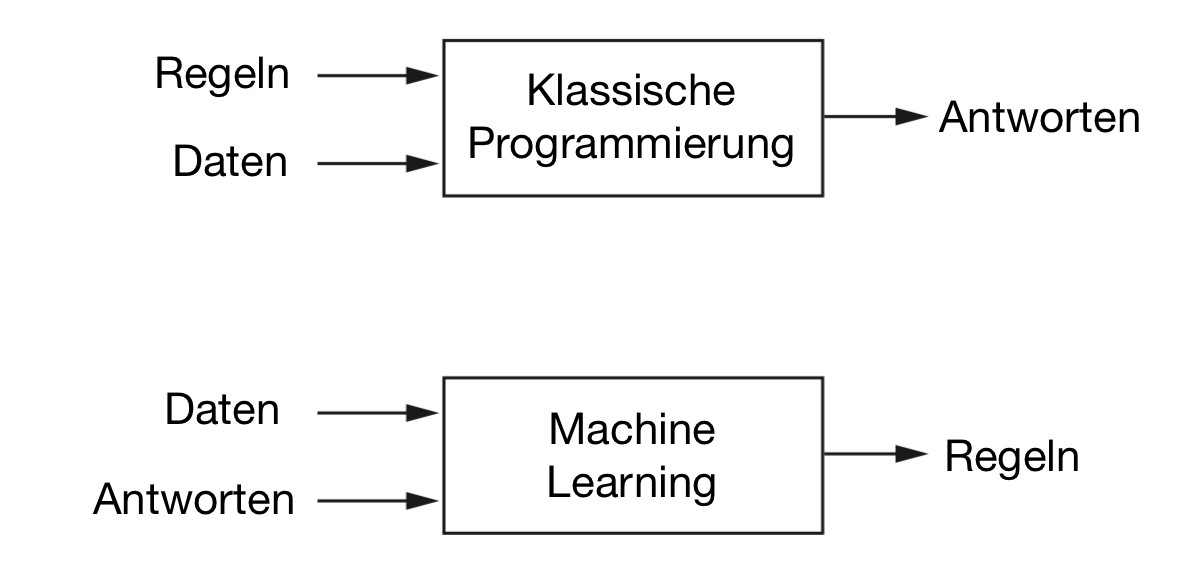
\includegraphics[width=15cm, height=6.5cm]{Abbildung_MaschinellesLernen_1.jpg}
	\caption{Maschinelles Lernen vs. Klassische Programmierung}
	\label{fig1}
\end{figure}

In der Abbildung 1, sehen wir den unterschied zwischen Klassische Programmierung und Maschinelle Lern Algorithmen. Bei den Klassischen Programmierung werden Regeln definiert und implementiert und anhand dieser Regeln werden die Daten verarbeitet, die dann zu einem Antwort führen. Anders ist es aber bei den Maschinelle Lernalgorithmen. Hier werden Daten und dessen Antworten als Inputdaten betrachtet, wodurch die Maschine für sich die Regeln definiert.

Um Entscheidungen zu treffen, werden Eingabedaten benötigt, die der Maschine die nötigen Informationen liefert. Die Eingabedaten beinhaltet auch die Lösung des Problems und somit auch den Wert, der von der Maschine vorhergesagt werden soll. Damit die Maschine nach Effizienz bewertet werden kann, ist eine Messung der Algorithmen erforderlich.

Für die Lösungen der Probleme werden verschiedentliche Maschinelle Lernalgorithmen verwenden. Die Entscheidung welches benutzt werden soll hängt von den Eingabedaten und das Ziel ab. Im Rahmen dieser Arbeit, liegt der Fokus auf das Convutional Neural Network verfahren, welches zu Kategorie des unüberwachten Lernen gehört.

\section{Unüberwachtes Lernen}

Das Ziel des Unüberwachten Lernens ist die Zusammenfassung oder auch Segmentierung der ähnliche Datenpunkte in Gruppen und gehört zu eine der vier Verfahren aus dem Maschinelle Lern Algorithmen. Die Maschine erhält während dem Lernvorgang nur die Eingabedaten ohne die zu erwartenden Ergebnisse, dadurch werden die Daten, die sich den anderen Datenpunkten statisch ähnlich sind, segmentiert. Die Segmentierung wird auch benutzt, um große Datensätze auf die Klassifizierung vorzubereiten. Diesbezüglich wird aus den Datenpunkten einer Gruppe eine Stichprobe genutzt. Es ist möglich das Gruppen auch falsch zugeordnet werden, somit wird ein gewisses Risiko eingegangen, dies wird durch eine hohe Anzahl an Stichproben verringert.

\section{Neuronale Netze}

\section{Deep Learning}

\begin{figure}[ht]
	\centering
  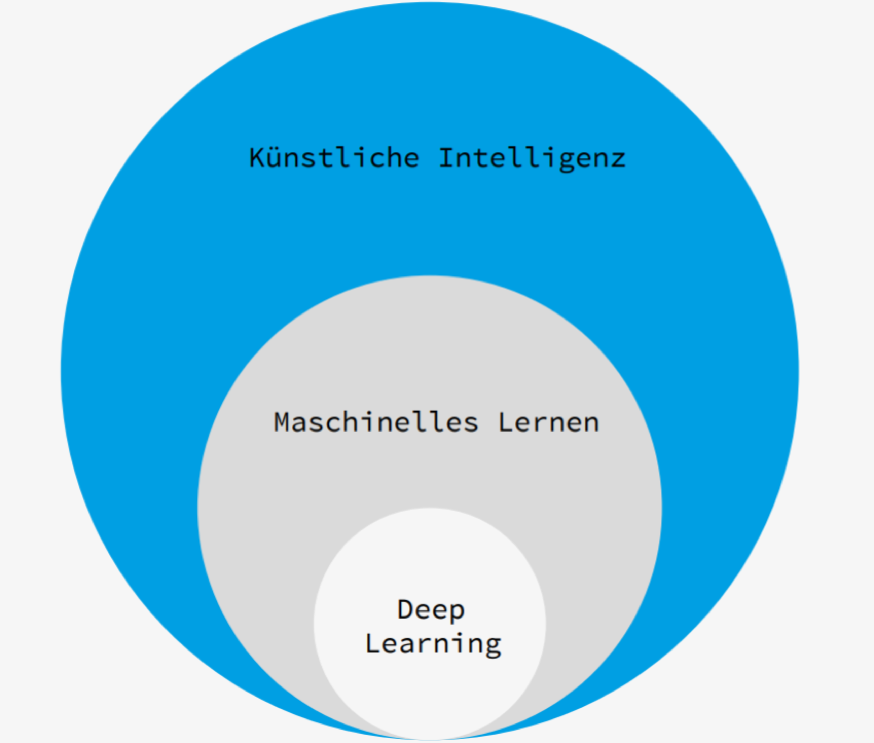
\includegraphics[width=10cm,height=6.5cm]{Abbildung_DeepLearning_1.png}
	\caption{Obermenge des Deep Learnings}
	\label{fig2}
\end{figure}

Wie im Abbildung 2 zu sehen ist, ist die Deep Learning eine Teilmenge der Maschinelle Lernalgorithmen, welches zu der Kategorie des unüberwachte Lernens gehört.

\section{CNN}

\section{CRIPS-DM Modell}

\section{Bisherige Arbeiten}

\section{Fazit}

\end{document}